%%%%%%%%%%%%%%%%%%%%%%%%%%%%%%%%%%%%%%%%%%%%%%%%%%%%%%%%%%%%%%%%%%%%%%%%%%%
\chapter{Introduction}
%%%%%%%%%%%%%%%%%%%%%%%%%%%%%%%%%%%%%%%%%%%%%%%%%%%%%%%%%%%%%%%%%%%%%%%%%%%

Functional programming has suddenly risen to popularity 
with examples that include Scala, Clojure, ReactJS, and 
other languages adopting lambda expressions. Reasoning 
about program correctness in a pure function can be done 
in a dependently-typed, proof assistant such as Coq or 
Agda\cite{Breitner2018}\cite{SpectorZabusky2018}\cite{ElBakouny2017}. 
Likewise, pure functions can be easily proved by using 
induction. Composing two proven functions into a single 
function should also give the correct result\cite{AbelBenkeBove2005}.

This research aims to utilize the existing A* pathfinding 
algorithm\cite{ZaghloulAlJami2017}\cite{WeinstockHolladay}
and find a way to develop a reasonably-efficient 
purely functional implementation of the algorithm using parallel 
data structures such as STMs or MVars\cite{Marlow2013}.  
The main objective of the research is 
to find an efficient concurrent implementation of a maze solver 
in a purely functional programming environment with comparable 
performance and space complexity of a performant imperative 
programming language.

% The Shortest Common Superstring (SCS) problem, known to be NP-Complete,
% seeks the shortest string that contains all strings from a given set.
% In this paper, we provide the summary of the problem and some of its characteristics.

% The SCS problem has been extensively studied for its
% applications in string compression and DNA sequence assembly \cite{Ma2009}.

% The superstring problem has applications to data storage,
%  specifically, data (string) compression \cite{Gallant1980}. 
% In many programming languages, a character string may be 
% represented by a pointer to that string. 
% The problem for the compiler is to arrange strings 
% so that they may be ``overlapped'' as much as possible.

% DNA sequence assembly is another  problem to which an SCS algorithm is known to apply.
% The $sequencing$ problem in molecular biology is to ``read'' a string of DNA,
% which can be viewed as a string over the alphabet \{A,C,G,T\}. Sequencing produces such a large number of fragments that
% almost all genome positions are covered by many fragments. This short fragments
% thus have large overlaps between other pieces. Hence, they can be given as an input to SCS algorithm.
% Figure \ref{fig:dna-overlap} shows an overlap graph consisting DNA reads (or fragments) as nodes. 



% \begin{figure*}
% \centering
% \fbox{
% \scalebox{0.65}{
% 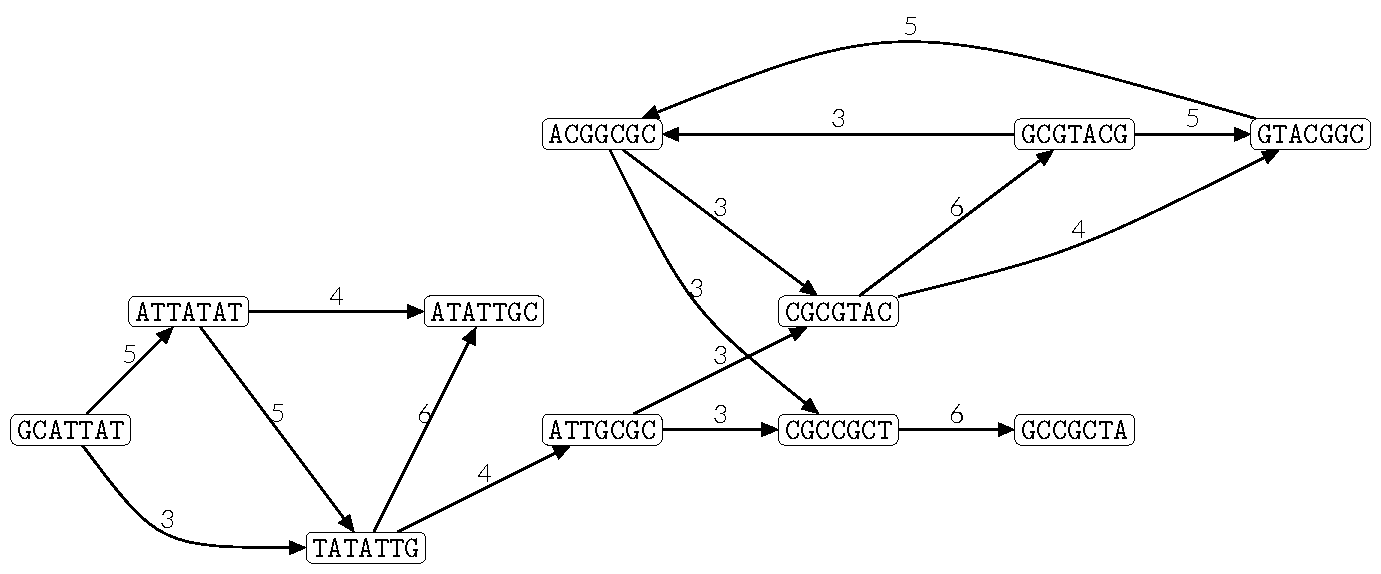
\includegraphics{fig-overlaps-dns-example}
% }}
% \caption{Sample overlap graph with each adjacent nodes 
% having at least $k = 3$ overlaps. The original string is \texttt{GCATTATATATTGCGCGTACGGCGCCGCTACA}.}
% \label{fig:dna-overlap}
% \end{figure*}	

% In \cite{Ma2009}'s paper, SCS was used to analyze DNA sequence assembly using
% a greedy algorithm. 

% \section{Project Context}

% \section{Purpose and Description}

% \section{Objectives}

% \vfill\eject
\section{Scope and Limitations}
The researchers will utilize Haskell for concrete implementation 
of the parallel A* algorithm in a functional programming environment.
Likewise, for performance comparison, the researchers 
will use the Rust programming language due to some of its features having
similarities with Haskell such as correct concurrent programs\cite{Saligrama2019}
and guarantees a relatively safe program\cite{Jung2018}.

Other purely-functional languages or lambda notation for generality
will not be used. Other concurrent data structures besides \verb|MVar| and Software
Transactional Memory will not be utilized.